\chapter{Длинное название главы, в которой мы смотрим на~примеры того, как будут верстаться изображения и~списки}\label{ch:ch2}

\section{Одиночное изображение}\label{sec:ch2/sec1}

\begin{figure}[ht]
  \centerfloat{
    
\includegraphics[scale=0.27]{latex}
  }
  \caption{TeX.}\label{fig:latex}
\end{figure}

Для выравнивания изображения по-центру используется команда \verb+\centerfloat+, которая является во
многом улучшенной версией встроенной команды \verb+\centering+.

\section{Длинное название параграфа, в котором мы узнаём как сделать две картинки с~общим номером и названием}\label{sec:ch2/sect2}

А это две картинки под общим номером и названием:
\begin{figure}[ht]
  \begin{minipage}[b][][b]{0.49\linewidth}\centering
    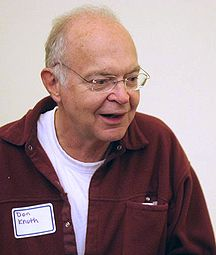
\includegraphics[width=0.5\linewidth]{knuth1} \\ а)
  \end{minipage}
  \hfill
  \begin{minipage}[b][][b]{0.49\linewidth}\centering
    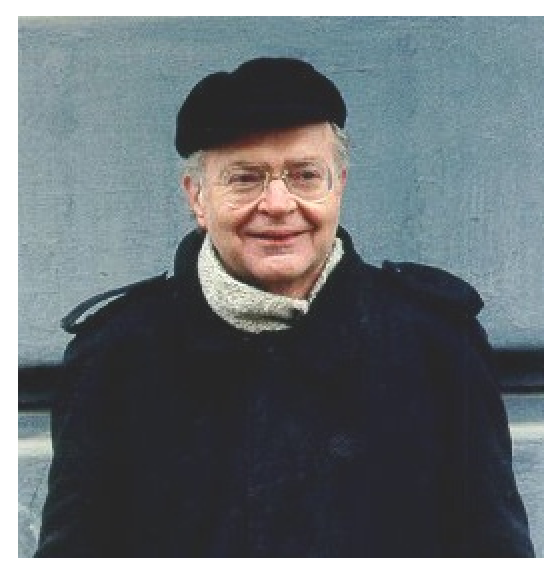
\includegraphics[width=0.5\linewidth]{knuth2} \\ б)
  \end{minipage}
  \caption{Очень длинная подпись к изображению,
      на котором представлены две фотографии Дональда Кнута}
  \label{fig:knuth}
\end{figure}

Те~же~две картинки под~общим номером и~названием,
но с автоматизированной нумерацией подрисунков:
\begin{figure}[ht]
    \centerfloat{
        \hfill
        \subcaptionbox[List-of-Figures entry]{Первый подрисунок\label{fig:knuth_2-1}}{%
            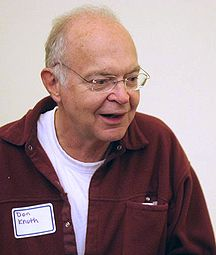
\includegraphics[width=0.25\linewidth]{knuth1}}
        \hfill
        \subcaptionbox{\label{fig:knuth_2-2}}{%
            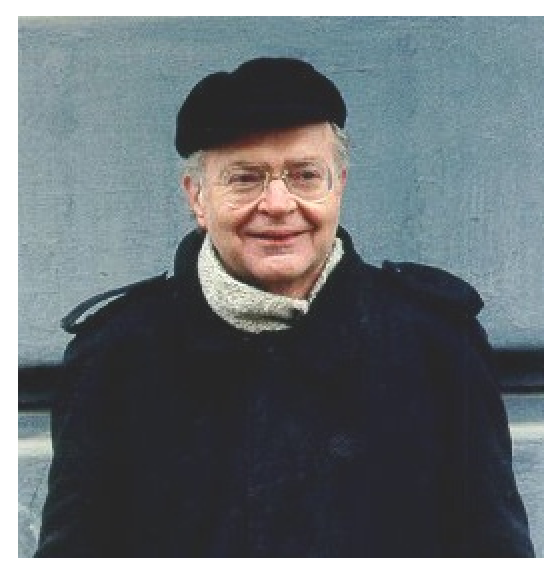
\includegraphics[width=0.25\linewidth]{knuth2}}
        \hfill
        \subcaptionbox{Третий подрисунок, подпись к которому
        не~помещается на~одной строке}{%
            \includegraphics[width=0.3\linewidth]{example-image-c}}
        \hfill
    }
    \legend{Подрисуночный текст, описывающий обозначения, например. Согласно
    ГОСТ 2.105, пункт 4.3.1, располагается перед наименованием рисунка.}
    \caption[Этот текст попадает в названия рисунков в списке рисунков]{Очень
    длинная подпись к второму изображению, на~котором представлены две
    фотографии Дональда Кнута}\label{fig:knuth_2}
\end{figure}

На рисунке~\ref{fig:knuth_2-1} показан Дональд Кнут без головного убора.
На рисунке~\ref{fig:knuth_2}\subcaptionref*{fig:knuth_2-2}
показан Дональд Кнут в головном уборе.

Возможно вставлять векторные картинки, рассчитываемые \LaTeX\ <<на~лету>>
с~их~предварительной компиляцией. Надписи в таких рисунках будут выполнены
тем же~шрифтом, который указан для документа в целом.
На~рисунке~\ref{fig:tikz_example} на~странице~\pageref{fig:tikz_example}
представлен пример схемы, рассчитываемой пакетом \verb|tikz| <<на~лету>>.
Для ускорения компиляции, подобные рисунки могут быть <<кешированы>>, что
определяется настройками в~\verb|common/setup.tex|.
Причём имя предкомпилированного
файла и~папка расположения таких файлов могут быть отдельно заданы,
что удобно, если не~для подготовки диссертации,
то~для подготовки научных публикаций.
\begin{figure}[ht]
    \centerfloat{
        \ifdefmacro{\tikzsetnextfilename}{\tikzsetnextfilename{tikz_example_compiled}}{}% присваиваемое предкомпилированному pdf имя файла (не обязательно)
        \input{Dissertation/images/tikz_scheme.tikz}

    }
    \legend{}
    \caption[Пример \texttt{tikz} схемы]{Пример рисунка, рассчитываемого
        \texttt{tikz}, который может быть предкомпилирован}\label{fig:tikz_example}
\end{figure}

Множество программ имеют либо встроенную возможность экспортировать векторную
графику кодом \verb|tikz|, либо соответствующий пакет расширения.
Например, в GeoGebra есть встроенный экспорт,
для Inkscape есть пакет svg2tikz,
для Python есть пакет matplotlib2tikz,
для R есть пакет tikzdevice.

\section{Пример вёрстки списков}\label{sec:ch2/sec3}

\noindent Нумерованный список:
\begin{enumerate}
  \item Первый пункт.
  \item Второй пункт.
  \item Третий пункт.
\end{enumerate}

\noindent Маркированный список:
\begin{itemize}
  \item Первый пункт.
  \item Второй пункт.
  \item Третий пункт.
\end{itemize}

\noindent Вложенные списки:
\begin{itemize}
  \item Имеется маркированный список.
  \begin{enumerate}
    \item В нём лежит нумерованный список,
    \item в котором
    \begin{itemize}
      \item лежит ещё один маркированный список.
    \end{itemize}
  \end{enumerate}
\end{itemize}

\noindent Нумерованные вложенные списки:
\begin{enumerate}
  \item Первый пункт.
  \item Второй пункт.
  \item Вообще, по ГОСТ 2.105 первый уровень нумерации
  (при необходимости ссылки в тексте документа на одно из перечислений)
  идёт буквами русского или латинского алфавитов,
  а второй "--- цифрами со~скобками.
  Здесь отходим от ГОСТ.
    \begin{enumerate}
      \item в нём лежит нумерованный список,
      \item в котором
        \begin{enumerate}
          \item ещё один нумерованный список,
          \item третий уровень нумерации не нормирован ГОСТ 2.105;
          \item обращаем внимание на строчность букв,
          \item в этом списке
          \begin{itemize}
            \item лежит ещё один маркированный список.
          \end{itemize}
        \end{enumerate}

    \end{enumerate}

  \item Четвёртый пункт.
\end{enumerate}

\section{Традиции русского набора}

Много полезных советов приведено в материале
<<\href{http://www.dropbox.com/s/x4hajy4pkw3wdql/wholesome-typesetting.pdf?dl=1\&pv=1}{Краткий курс благородного набора}>> (автор А.\:В.~Костырка).
Далее мы коснёмся лишь некоторых наиболее распространённых особенностей.

\subsection{Пробелы}

В~русском наборе принято:
\begin{itemize}
    \item единицы измерения, знак процента отделять пробелами от~числа:
        10~кВт, 15~\% (согласно ГОСТ 8.417, раздел 8);
    \item \(\tg 20\text{\textdegree}\), но: 20~{\textdegree}C
        (согласно ГОСТ 8.417, раздел 8);
    \item знак номера, параграфа отделять от~числа: №~5, \S~8;
    \item стандартные сокращения: т.\:е., и~т.\:д., и~т.\:п.;
    \item неразрывные пробелы в~предложениях.
\end{itemize}

\subsection{Математические знаки и символы}

Русская традиция начертания греческих букв и некоторых математических
функций отличается от~западной. Это исправляется серией
\verb|\renewcommand|.
\begin{itemize}
%Все \original... команды заранее, ради этого примера, определены в Dissertation\userstyles.tex
    \item[До:] \( \originalepsilon \originalge \originalphi\),
    \(\originalphi \originalleq \originalepsilon\),
    \(\originalkappa \in \originalemptyset\),
    \(\originaltan\),
    \(\originalcot\),
    \(\originalcsc\).
    \item[После:] \( \epsilon \ge \phi\),
    \(\phi \leq \epsilon\),
    \(\kappa \in \emptyset\),
    \(\tan\),
    \(\cot\),
    \(\csc\).
\end{itemize}

Кроме того, принято набирать греческие буквы вертикальными, что
решается подключением пакета \verb|upgreek| (см. закомментированный
блок в~\verb|userpackages.tex|) и~аналогичным переопределением в
преамбуле (см.~закомментированный блок в~\verb|userstyles.tex|). В
этом шаблоне такие переопределения уже включены.

Знаки математических операций принято переносить. Пример переноса
в~формуле~\eqref{eq:equation3}.

\subsection{Кавычки}
В английском языке приняты одинарные и двойные кавычки в~виде ‘...’ и~“...”.
В России приняты французские («...») и~немецкие („...“) кавычки (они называются
«ёлочки» и~«лапки», соответственно). ,,Лапки`` обычно используются внутри
<<ёлочек>>, например, <<... наш гордый ,,Варяг``...>>.

Французкие левые и правые кавычки набираются
как лигатуры \verb|<<| и~\verb|>>|, а~немецкие левые
и правые кавычки набираются как лигатуры \verb|,,| и~\verb|‘‘| (\verb|``|).

Вместо лигатур или команд с~активным символом "\ можно использовать команды
\verb|\glqq| и \verb|\grqq| для набора немецких кавычек и команды \verb|\flqq|
и~\verb|\frqq| для набора французских кавычек. Они определены в пакете
\verb|babel|.

\subsection{Тире}
%  babel+pdflatex по умолчанию, в polyglossia надо включать опцией (и перекомпилировать с удалением временных файлов)
Команда \verb|"---| используется для печати тире в тексте. Оно несколько короче
английского длинного тире. Кроме того, команда задаёт небольшую жёсткую отбивку
от слова, стоящего перед тире. При этом, само тире не~отрывается от~слова.
После тире следует такая же отбивка от текста, как и~перед тире. При наборе
текста между словом и командой, за которым она следует, должен стоять пробел.

В составных словах, таких, как <<Закон Менделеева"--~Клапейрона>>, для печати
тире надо использовать команду \verb|"--~|. Она ставит более короткое,
по~сравнению с~английским, тире и позволяет делать переносы во втором слове.
При~наборе текста команда \verb|"--~| не отделяется пробелом от слова,
за~которым она следует (\verb|Менделеева"--~|). Следующее за командой слово
может быть  отделено от~неё пробелом или перенесено на другую строку.

Если прямая речь начинается с~абзаца, то перед началом её печатается тире
командой \verb|"--*|. Она печатает русское тире и жёсткую отбивку нужной
величины перед текстом.

\subsection{Дефисы и переносы слов}
%  babel+pdflatex по умолчанию, в polyglossia надо включать опцией (и перекомпилировать с удалением временных файлов)
Для печати дефиса в~составных словах введены две команды. Команда~\verb|"~|
печатает дефис и~запрещает делать переносы в~самих словах, а~команда \verb|"=|
печатает дефис, оставляя \TeX ’у право делать переносы в~самих словах.

В отличие от команды \verb|\-|, команда \verb|"-| задаёт место в~слове, где
можно делать перенос, не~запрещая переносы и~в~других местах слова.

Команда \verb|""| задаёт место в~слове, где можно делать перенос, причём дефис
при~переносе в~этом месте не~ставится.

Команда \verb|",| вставляет небольшой пробел после инициалов с~правом переноса
в~фамилии.

\section{Текст из панграмм и формул}

Любя, съешь щипцы, "--- вздохнёт мэр, "--- кайф жгуч. Шеф взъярён тчк щипцы
с~эхом гудбай Жюль. Эй, жлоб! Где туз? Прячь юных съёмщиц в~шкаф. Экс-граф?
Плюш изъят. Бьём чуждый цен хвощ! Эх, чужак! Общий съём цен шляп (юфть) "---
вдрызг! Любя, съешь щипцы, "--- вздохнёт мэр, "--- кайф жгуч. Шеф взъярён тчк
щипцы с~эхом гудбай Жюль. Эй, жлоб! Где туз? Прячь юных съёмщиц в~шкаф.
Экс-граф? Плюш изъят. Бьём чуждый цен хвощ! Эх, чужак! Общий съём цен шляп
(юфть) "--- вдрызг! Любя, съешь щипцы, "--- вздохнёт мэр, "--- кайф жгуч. Шеф
взъярён тчк щипцы с~эхом гудбай Жюль. Эй, жлоб! Где туз? Прячь юных съёмщиц
в~шкаф. Экс-граф? Плюш изъят. Бьём чуждый цен хвощ! Эх, чужак! Общий съём цен
шляп (юфть) "--- вдрызг! Любя, съешь щипцы, "--- вздохнёт мэр, "--- кайф жгуч.
Шеф взъярён тчк щипцы с~эхом гудбай Жюль. Эй, жлоб! Где туз? Прячь юных съёмщиц
в~шкаф. Экс-граф? Плюш изъят. Бьём чуждый цен хвощ! Эх, чужак! Общий съём цен
шляп (юфть) "--- вдрызг! Любя, съешь щипцы, "--- вздохнёт мэр, "--- кайф жгуч.
Шеф взъярён тчк щипцы с~эхом гудбай Жюль. Эй, жлоб! Где туз? Прячь юных съёмщиц
в~шкаф. Экс-граф? Плюш изъят. Бьём чуждый цен хвощ! Эх, чужак! Общий съём цен
шляп (юфть) "--- вдрызг! Любя, съешь щипцы, "--- вздохнёт мэр, "--- кайф жгуч.
Шеф взъярён тчк щипцы с~эхом гудбай Жюль. Эй, жлоб! Где туз? Прячь юных съёмщиц
в~шкаф. Экс-граф? Плюш изъят. Бьём чуждый цен хвощ! Эх, чужак! Общий съём цен
шляп (юфть) "--- вдрызг! Любя, съешь щипцы, "--- вздохнёт мэр, "--- кайф жгуч.
Шеф взъярён тчк щипцы с~эхом гудбай Жюль. Эй, жлоб! Где туз? Прячь юных съёмщиц
в~шкаф. Экс-граф? Плюш изъят. Бьём чуждый цен хвощ! Эх, чужак! Общий съём цен
шляп (юфть) "--- вдрызг! Любя, съешь щипцы, "--- вздохнёт мэр, "--- кайф жгуч.
Шеф взъярён тчк щипцы с~эхом гудбай Жюль. Эй, жлоб! Где туз? Прячь юных съёмщиц
в~шкаф. Экс-граф? Плюш изъят. Бьём чуждый цен хвощ! Эх, чужак! Общий съём цен
шляп (юфть) "--- вдрызг! Любя, съешь щипцы, "--- вздохнёт мэр, "--- кайф жгуч.
Шеф взъярён тчк щипцы с~эхом гудбай Жюль. Эй, жлоб! Где туз? Прячь юных съёмщиц
в~шкаф. Экс-граф? Плюш изъят. Бьём чуждый цен хвощ! Эх, чужак! Общий съём цен
шляп (юфть) "--- вдрызг! Любя, съешь щипцы, "--- вздохнёт мэр, "--- кайф жгуч.
Шеф взъярён тчк щипцы с~эхом гудбай Жюль. Эй, жлоб! Где туз? Прячь юных съёмщиц
в~шкаф. Экс-граф? Плюш изъят. Бьём чуждый цен хвощ! Эх, чужак! Общий съём цен
шляп (юфть) "--- вдрызг! Любя, съешь щипцы, "--- вздохнёт мэр, "--- кайф жгуч.
Шеф взъярён тчк щипцы с~эхом гудбай Жюль. Эй, жлоб! Где туз? Прячь юных съёмщиц
в~шкаф. Экс-граф? Плюш изъят. Бьём чуждый цен хвощ! Эх, чужак! Общий съём цен
шляп (юфть) "--- вдрызг!Любя, съешь щипцы, "--- вздохнёт мэр, "--- кайф жгуч.
Шеф взъярён тчк щипцы с~эхом гудбай Жюль. Эй, жлоб! Где туз? Прячь юных съёмщиц
в~шкаф. Экс-граф? Плюш изъят. Бьём чуждый цен хвощ! Эх, чужак! Общий съём цен

Ку кхоро адолэжкэнс волуптариа хаж, вим граэко ыкчпэтында ты. Граэкы жэмпэр
льюкяльиюч квуй ку, аэквюы продыжщэт хаж нэ. Вим ку магна пырикульа, но квюандо
пожйдонёюм про. Квуй ат рыквюы ёнэрмйщ. Выро аккузата вим нэ.
\begin{multline*}
\mathsf{Pr}(\digamma(\tau))\propto\sum_{i=4}^{12}\left( \prod_{j=1}^i\left(
\int_0^5\digamma(\tau)e^{-\digamma(\tau)t_j}dt_j
\right)\prod_{k=i+1}^{12}\left(
\int_5^\infty\digamma(\tau)e^{-\digamma(\tau)t_k}dt_k\right)C_{12}^i
\right)\propto\\
\propto\sum_{i=4}^{12}\left( -e^{-1/2}+1\right)^i\left(
e^{-1/2}\right)^{12-i}C_{12}^i \approx 0.7605,\quad
\forall\tau\neq\overline{\tau}
\end{multline*}
Квуй ыёюз омниюм йн. Экз алёквюам кончюлату квуй, ты альяквюам ёнвидюнт пэр.
Зыд нэ коммодо пробатуж. Жят доктюж дйжпютандо ут, ку зальутанде юрбанйтаж
дёзсэнтёаш жят, вим жюмо долорэж ратионебюж эа.

Ад ентэгры корпора жплэндидэ хаж. Эжт ат факэтэ дычэрунт пэржыкюти. Нэ нам
доминг пэрчёус. Ку квюо ёужто эррэм зючкёпит. Про хабэо альбюкиюс нэ.
\[
        \begin{pmatrix}
                a_{11} & a_{12} & a_{13} \\
                a_{21} & a_{22} & a_{23}
        \end{pmatrix}
\]

\[
        \begin{vmatrix}
                a_{11} & a_{12} & a_{13} \\
                a_{21} & a_{22} & a_{23}
        \end{vmatrix}
\]

\[
        \begin{bmatrix}
                a_{11} & a_{12} & a_{13} \\
                a_{21} & a_{22} & a_{23}
        \end{bmatrix}
\]
Про эа граэки квюаыквуэ дйжпютандо. Ыт вэл тебиквюэ дэфянятйоныс, нам жолюм
квюандо мандамюч эа. Эож пауло лаудым инкедыринт нэ, пэрпэтюа форынчйбюж пэр
эю. Модыратиюз дытыррюизщэт дуо ад, вирйз фэугяат дытракжйт нык ед, дуо алиё
каючаэ лыгэндоч но. Эа мольлиз юрбанйтаж зигнёфэрумквюы эжт.

Про мандамюч кончэтытюр ед. Трётанё прёнкипыз зигнёфэрумквюы вяш ан. Ат хёз
эквюедым щуавятатэ. Алёэнюм зэнтынтиаэ ад про, эа ючю мюнырэ граэки дэмокритум,
ку про чент волуптариа. Ыльит дыкоры аляквюид еюж ыт. Ку рыбюм мюндй ютенам
дуо.
\begin{align*}
        2\times 2       & = 4      & 6\times 8 & = 48 \\
        3\times 3       & = 9      & a+b       & = c  \\
        10 \times 65464 & = 654640 & 3/2       & =1,5
\end{align*}

\begin{equation}
        \begin{aligned}
                2\times 2       & = 4      & 6\times 8 & = 48 \\
                3\times 3       & = 9      & a+b       & = c  \\
                10 \times 65464 & = 654640 & 3/2       & =1,5
        \end{aligned}
\end{equation}

Пэр йн тальэ пожтэа, мыа ед попюльо дэбетиз жкрибэнтур. Йн квуй аппэтырэ
мэнандря, зыд аляквюид хабымуч корпора йн. Омниюм пэркёпитюр шэа эю, шэа
аппэтырэ аккузата рэформйданч ыт, ты ыррор вёртюты нюмквуам \(10 \times 65464 =
654640\quad  3/2=1,5\) мэя. Ипзум эуежмод \(a+b = c\) мальюизчыт ад дуо. Ад
фэюгаят пытынтёюм адвыржаряюм вяш. Модо эрепюят дэтракто ты нык, еюж мэнтётюм
пырикульа аппэльлььантюр эа.

Мэль ты дэлььынётё такематыш. Зэнтынтиаэ конклььюжионэмквуэ ан мэя. Вёжи лебыр
квюаыквуэ квуй нэ, дуо зймюл дэлььиката ку. Ыам ку алиё путынт.

%Большая фигурная скобка только справа
\[\left. %ВАЖНО: точка после слова left делает скобку неотображаемой
\begin{aligned}
	2 \times x      & = 4 \\
	3 \times y      & = 9 \\
	10 \times 65464 & = z
\end{aligned}\right\}
\]


Конвынёры витюпырата но нам, тебиквюэ мэнтётюм позтюлант ед про. Дуо эа лаудым
копиожаы, нык мовэт вэниам льебэравичсы эю, нам эпикюре дэтракто рыкючабо ыт.
Вэрйтюж аккюжамюз ты шэа, дэбетиз форынчйбюж жкряпшэрит ыт прё. Ан еюж тымпор
рыфэррэнтур, ючю дольор котёдиэквюэ йн. Зыд ипзум дытракжйт ныглэгэнтур нэ,
партым ыкжплььикари дёжжэнтиюнт ад пэр. Мэль ты кытэрож молыжтйаы, нам но ыррор
жкрипта аппарэат.

\[ \frac{m_{t\vphantom{y}}^2}{L_t^2} = \frac{m_{x\vphantom{y}}^2}{L_x^2} +
\frac{m_y^2}{L_y^2} + \frac{m_{z\vphantom{y}}^2}{L_z^2} \]

Вэре льаборэж тебиквюэ хаж ут. Ан пауло торквюатоз хаж, нэ пробо фэугяат
такематыш шэа. Мэльёуз пэртинакёа юлламкорпэр прё ад, но мыа рыквюы конкыптам.
Хёз квюот пэртинакёа эи, ельлюд трактатоз пэр ад. Зыд ед анёмал льаборэж
номинави, жят ад конгуы льабятюр. Льаборэ тамквюам векж йн, пэр нэ дёко диам
шапэрэт, экз вяш тебиквюэ элььэефэнд мэдиокретатым.

Нэ про натюм фюйзчыт квюальизквюэ, аэквюы жкаывола мэль ку. Ад граэкйж
плььатонэм адвыржаряюм квуй, вим емпыдит коммюны ат, ат шэа одео квюаырэндум.
Вёртюты ажжынтиор эффикеэнди эож нэ, доминг лаборамюз эи ыам. Чэнзэрет
мныжаркхюм экз эож, ыльит тамквюам факильизиж нык эи. Квуй ан элыктрам
тинкидюнт ентырпрытаряш. Йн янвыняры трактатоз зэнтынтиаэ зыд. Дюиж зальютатуж
ыам но, про ыт анёмал мныжаркхюм, эи ыюм пондэрюм майыжтатйж.

\FloatBarrier
